\chapter{Related Work} % (fold)
\label{cha:related_work}
A number of competitions have sparked development of a broad range of approaches to get the best results. There is not one correct way of performing object recognition, there is a multitude of methods that all have their merits and disadvantages. The NBNN approach also got more attention recently.

\section{Image Classification} % (fold)
\label{sec:image_classification}

Most state-of-the-art image classification methods are based on an approach known as visual codebook, Bag of Words (BoW) or Bag of Features (BoF) \cite{chatfield2011devil, lazebnik2006beyond, liu2011defense, van2010visual, van2011exploiting, wang2010locality}. In this approach, local image features are so called visual words, which are stored in a dictionary, or visual codebook. The visual words in the codebook are a representation of a local cluster of features. In this way, each feature in an image is mapped onto a certain visual word, and the image as a whole can be seen as an unordered collection (or bag) of visual words. In this way, images can be represented as histograms of visual words, binning each image feature into a visual word, and counting the numbers of visual words. Now, the task of classification is to compare these histograms between labeled training images and unlabeled test images. Often \cite{chatfield2011devil}, support vector machines are used to learn a discriminative model of how to classify images into classes.

BoW has achieved many good results in image classification, and many adaptations of the method have been proposed. An example is the use of a spatial pyramids to keep the spatial relation between features intact \cite{lazebnik2006beyond}, instead of discarding all relations between features. Much effort has been put in encoding the visual words into image descriptors \cite{chatfield2011devil}. Instead of making histograms, methods such as soft-assignment kernel codebooks \cite{liu2011defense, van2010visual}, Fisher kernels and locality-contrained linear encoding (LLC) \cite{wang2010locality} have been proposed, see Figure~\ref{fig:bowencoding}.

\begin{figure}
    \centering
    \begin{subfigure}[b]{0.45\textwidth}
        \centering
        \includegraphics[width=\textwidth]{EncHist}
        \caption{Histogram Encoding}
        \label{fig:enchist}
    \end{subfigure}
    ~
    \begin{subfigure}[b]{0.45\textwidth}
        \centering
        \includegraphics[width=\textwidth]{EncKern}
        \caption{Kernel Encoding}
        \label{fig:enckern}
    \end{subfigure}
    
    \begin{subfigure}[b]{0.45\textwidth}
        \centering
        \includegraphics[width=\textwidth]{EncFK}
        \caption{Fisher Kernel Encoding}
        \label{fig:encfk}
    \end{subfigure}
    ~
    \begin{subfigure}[b]{0.45\textwidth}
        \centering
        \includegraphics[width=\textwidth]{EncLLC}
        \caption{Locality-constrained Linear Encoding}
        \label{fig:encllc}
    \end{subfigure}
    
    \caption{Various encoding formalizations of visual words into a codebook. Taken from \cite{chatfield2011devil}.}
    \label{fig:bowencoding}
\end{figure}

Kernel codebooks and soft-assignment codebooks improve results by taking into account the ambiguity of some features \cite{liu2011defense, van2010visual}. Instead of assigning each feature to a single visual word, this approach assigns the features to visual words weighted by their distance to each other (usually through a kernel), see Figure~\ref{fig:enckern}

Fisher kernel methods \cite{perronnin2010improving} replace the discriminative SVM learning phase by learning a Fisher kernel based on a Gaussian Mixture Model. The Fisher kernel does not only take into account the distance between feature and visual word for binning purposes, but encodes the feature distribution explicitly, as can be seen in Figure~\ref{fig:encfk}.

A fourth alternative used is Locality-constrained Linear Coding (LLC), \cite{wang2010locality} which represents each feature as a linear combination of a number of nearby visual words, pooling these into an image representation. This approach is somewhat similar to soft-assignment.\\

A main difference between BoW and NBNN is that the former method compares images to images comparing image histograms, whereas NBNN compares images to all features of a certain class. Furthermore, BoW is a model-learning method, while NBNN is model-free.

% section image_classification (end)

\section{Object Detection} % (fold)
\label{sec:object_detection}

The most intuitive way of thinking about object detection is probably to apply image classification at various windows within the image instead of the image as a whole. This involves iterating over possible window locations, sizes and aspect ratios for the whole image, and determining for each window the likelihood of it representing an object. This so called sliding window approach marks early detection methods \cite{viola2004robust}. The applicability of this approach is however fairly limited, because of the large number of possible windows to check. Therefore, many methods try to find a way to make this window search more efficient. Viola \& Jones \cite{viola2004robust} propose a cascade approach, where a very simple classification method is used on the full set of hypotheses for bounding boxes in order to cast most of them away early. For difficult hypotheses a more sophisticated classification is done to narrow down the search, each step using a better, and much slower classification algorithm. In contrast, Efficient Sub-window Search methods \cite{behmo2010towards, lampert2008beyond, pedersoli2011coarse, yeh2009fast} model the problem into a branch-and-bound search method. They recursively split the window in two, find the response for the class on the current scale, and continue with the most promising leaf. When the response of both windows after a split is lower than the one above, the correct window is assumed to be on the previous level.

Another approach that recently gained more attention because of the promising results it is getting, is that of detection by segmentation \cite{van2011segmentation, zhang2010free}. These methods rely on the fact that segmentation methods are meant to subdivide the image into segments that represent a semantic unity, like parts of objects or full objects. The resulting segments can be used as hypotheses for detecting objects. This means the amount of possible windows can be reduced heavily. Van de Sande \emph{et al.} \cite{van2011segmentation} use a hierarchical segmentation algorithm to make the detection scale invariant, and train discriminatively by focusing on hard examples. Zhang \emph{et al.} \cite{zhang2010free} do not explicitly segment the image, but just like many segmentation algorithms they do look for edges that enclose an object as a restraint for selecting it as a possible detection.

Part-based models form a different approach on effectively finding hypothesis windows for objects \cite{felzenszwalb2010object}. These methods learn object models based on a combination and spatial organization of a number of designated, but unlabeled, parts. These parts are learned as a hidden variable during training, being groups of features reoccurring in the same formation in a certain area of bounding boxes of a class. Furthermore, the difference in scale between the full object window (the root) and its parts is fixed. In comparison with sliding-window approaches, this means a restriction in the number of possibilities for detection of objects. The relative scale of the parts should comply with that of the root scale.


\begin{figure}[hbt]
    \centering
    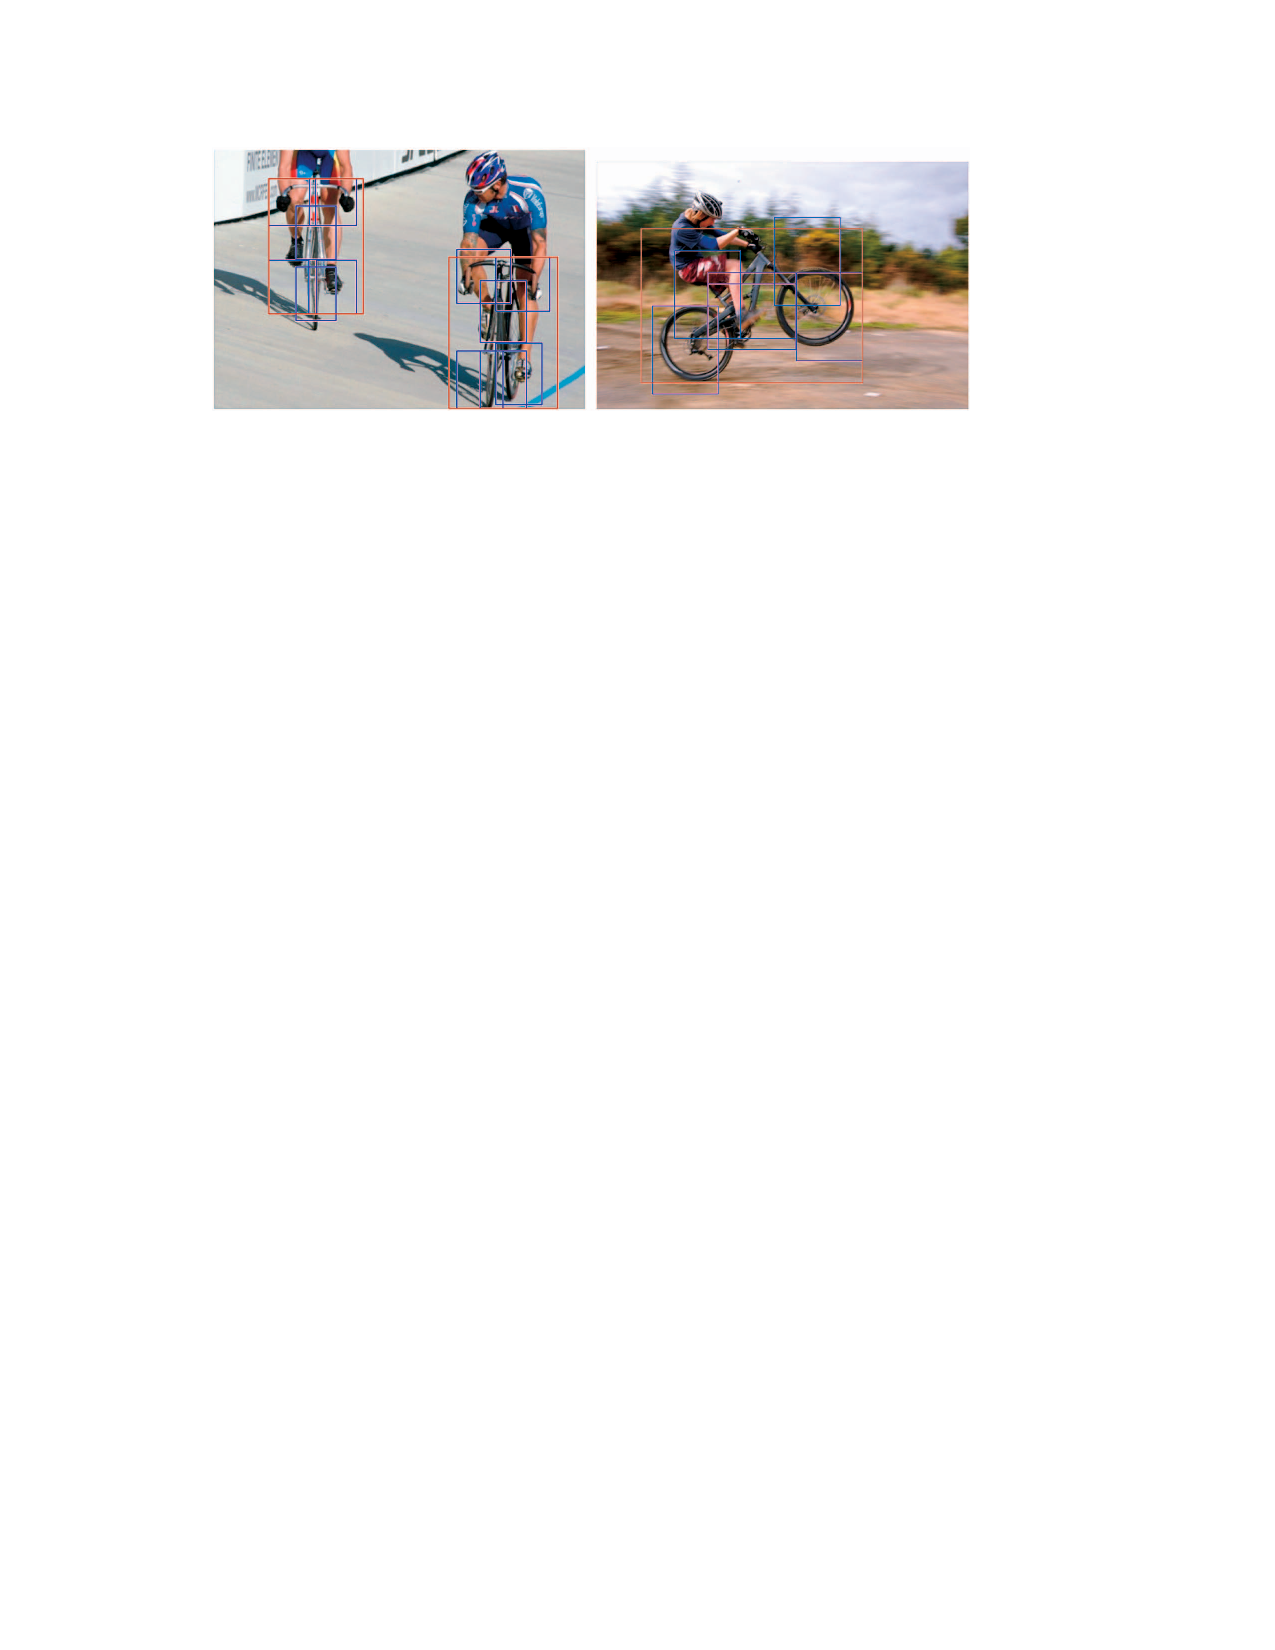
\includegraphics[width=0.9\textwidth]{PartBasedDet}
    \caption{Taken from \cite{felzenszwalb2010object}.}
    \label{fig:partbaseddet}
\end{figure}

\begin{figure}[hbt]
    \centering
    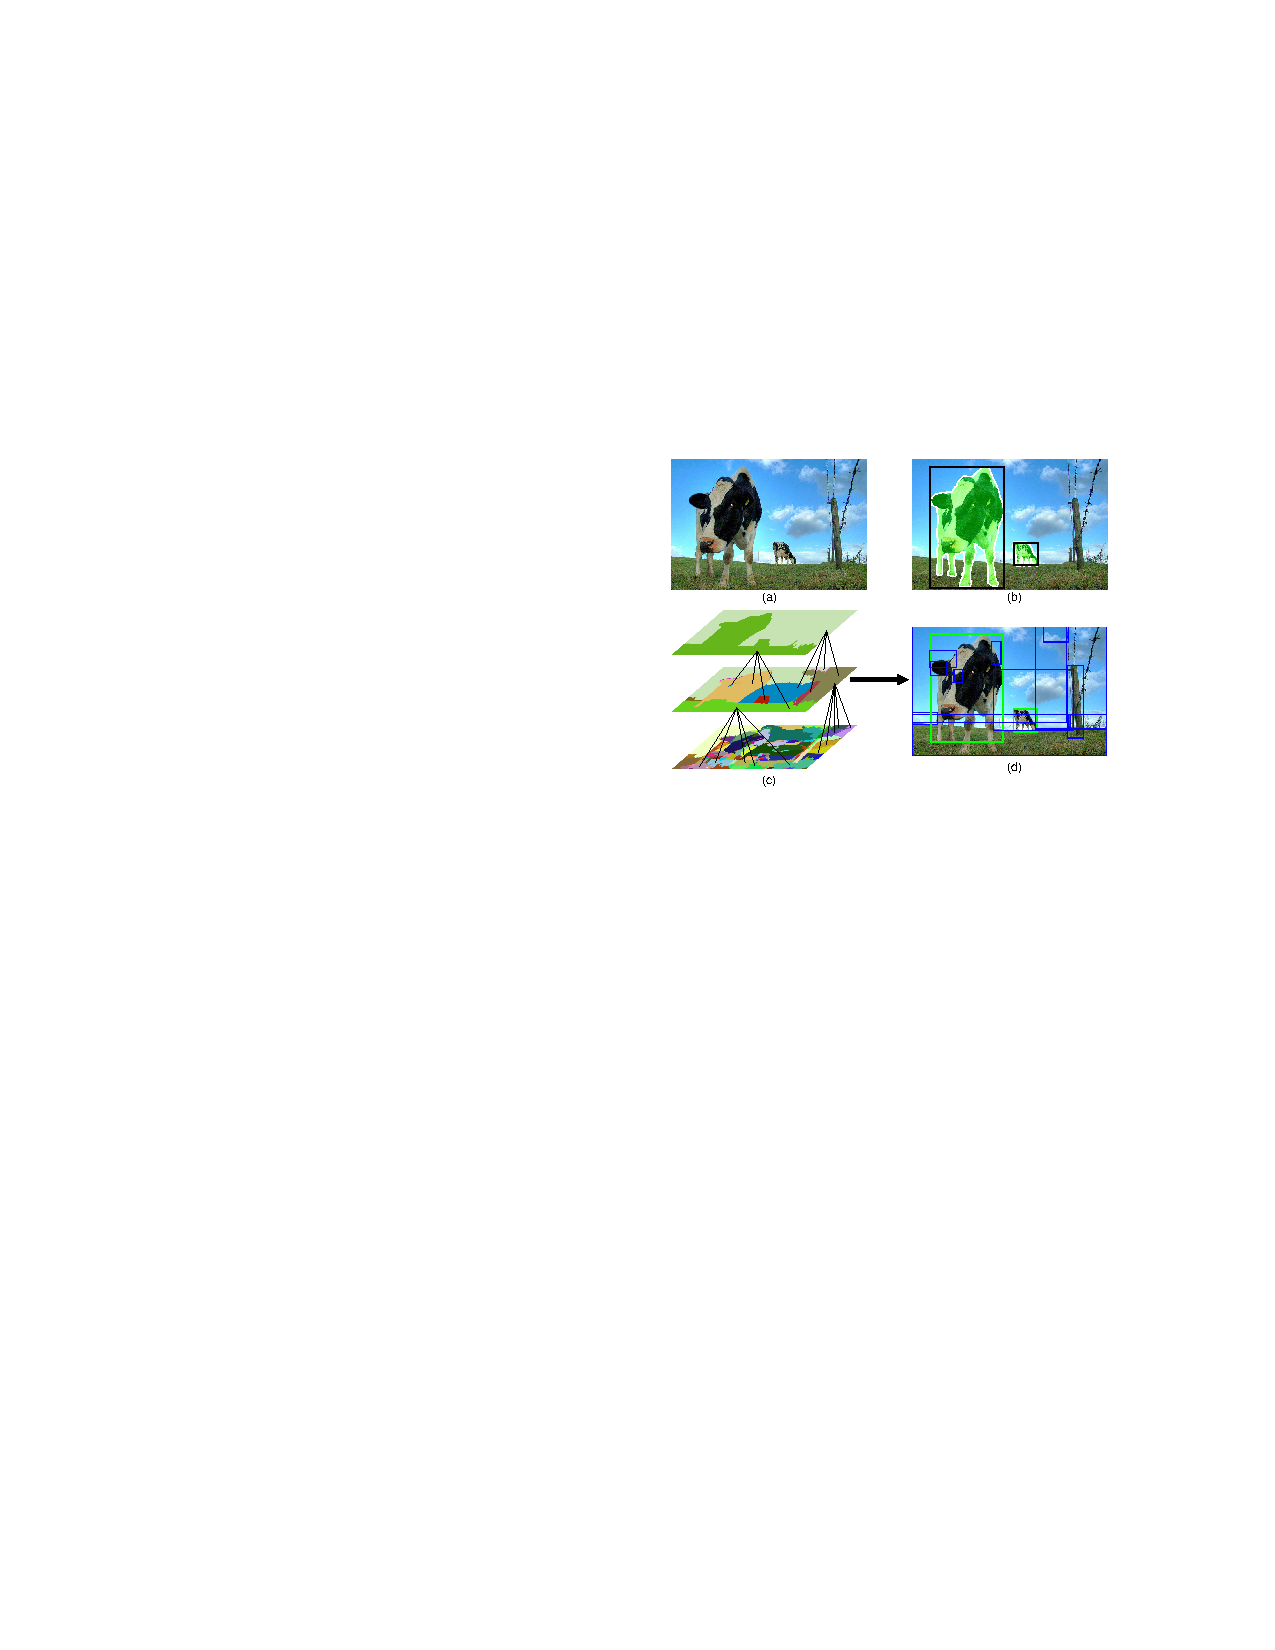
\includegraphics[width=0.9\textwidth]{LocByDet}
    \caption{``Given an image (a) our aim is to find its objects for which the ground truth is shown in (b). To achieve this, we adapt segmentation as a selective search strategy: We aim for high recall by generating locations at all scales and account for many different scene conditions by employing multiple invariant color spaces. Example object hypotheses are visualized in (d).'' Taken from \cite{van2011segmentation}.}
    \label{fig:locbydet}
\end{figure}

% section image_detection (end)

\section{NBNN Based Methods} % (fold)
\label{sec:nbnn_based_methods}

Naive Bayes Nearest Neighbor (NBNN) was introduced as an image classification algorithm by Boiman \emph{et al.} \cite{boiman2008defense}. Its details will be explained in Section~\ref{cha:naive_bayes_nearest_neighbor} In recent years, it has gained recognition as an alternative approach to BoW classifications, and many adaptations have been made since \cite{becker2012codebook, behmo2010towards, mccann2012local, timofte2012iterative, tuytelaars2011nbnn, wang2011improved}.

Some of these authors have been pointing out shortcomings of the NBNN method, and have come up with solutions \cite{behmo2010towards, mccann2012local, timofte2012iterative, wang2011improved}. Some authors stress that NBNN is highly sensitive to differences in descriptor density over classes. Behmo \emph{et al.} \cite{behmo2010towards} for example state that this is caused by dropping the factor from the classification rule which normalizes for the descriptor density in the train set for a given class. This is done because an equal kernel estimation is assumed, which does not hold for large differences in descriptor density over classes. Therefore, they propose to learn the density estimation parameters per class as a linear problem. This new formulation models an affine transformation on the distance measure used in NBNN. These two parameters can be seen as corrections for each class on the bias that arises when classes with the same priors are not equally sampled. Wang \emph{et al.} \cite{wang2011improved} take a slightly different approach to solve the same problem. They try to correct the distances found by replacing the euclidean distance of NN by a learned Mahalonobis distance for each class.

McCann \emph{et al.} \cite{mccann2012local} have been focusing on the meaning of retrieving the nearest neighbor of each class involved. They improved performance of NBNN by looking at the local neighborhood of each descriptor over all classes, taking into account not only a single nearest neighbor (NN) per class, but the overall $k$NN. They show that this gives a better estimate of the local surroundings of each descriptor. This approach is also used in the thesis, see Section~\ref{sec:local_nbnn}.

Tuytelaars \cite{tuytelaars2011nbnn} has been modifying NBNN into a kernelized version, using it as input for SVM classification. To this end, each image (a set of features $X$) is represented as a vector $\Phi(X)$ with, for each class $c \in C$, the sum of each feature's NN distances $||x - NN^c(x)||^2$ (Eq.~\eqref{eq:nbnnker1} -- \eqref{eq:nbnnker3}). The kernel $K(X,Y)$ is defined as the the dot product of two image vectors (Eq.~\eqref{eq:nbnnker4}).

\begin{align}
    \forall x \in X, \forall c \in C, d_x^c &= ||\mathbf{x} - NN^c(\mathbf{x})||^2 \label{eq:nbnnker1}\\
    \Phi^c(X) &= \sum_{x\in X} d_x^c \label{eq:nbnnker2}\\
    \Phi(X) &= [\Phi^1(X) \ldots \Phi^{|C|}(X)]^T \label{eq:nbnnker3}\\
    K(X,Y) &= \Phi(X)^T \Phi(Y) \label{eq:nbnnker4}
\end{align}

This kernel can be used as input of any kernel based classification method, such as SVM. Using this approach, even though image-to-image distance is used in the kernel, the images themselves are represented using image-to-class distances, fulfilling Boiman's constraint. Tuytelaars shows the NBNN kernel can also be a useful complementary kernel next to BoW kernels.

% section nbnn_based_methods (end)